% =============================================================================
% NER & Entity Resolution — an explanatory packet for step_7.
%
% Companion to stages/extract_entities.py (Tier-1 NER, Part B) and
% stages/resolve_entities.py (Tier-1 A3, the "grouping").
%
% Build (all aux/intermediary files land in build/, only .tex + .pdf stay here):
%     latexmk -pdf -outdir=build ner_and_resolution.tex
%     # then optionally:  cp build/ner_and_resolution.pdf .
%
% Wording follows the source-code comments closely, reorganised into prose with
% intuition first, then the mechanics, then caveats and sources.
% =============================================================================
\documentclass[11pt]{article}
\usepackage{lmodern}
\usepackage[T1]{fontenc}

% --- Packages ---------------------------------------------------------------
\usepackage[margin=1in]{geometry}
\usepackage{amsmath,amssymb}
\usepackage{microtype}
\microtypesetup{expansion=false}
\usepackage{enumitem}
\usepackage{booktabs}
\usepackage{graphicx}
\usepackage{xcolor}
\usepackage{hyperref}
\usepackage{listings}
\usepackage{tikz}
\usepackage[most]{tcolorbox}
\usepackage{placeins}   % \FloatBarrier keeps figures inside their section
\usepackage{caption}
\usetikzlibrary{arrows.meta, positioning, decorations.pathreplacing,
                calc, shapes.geometric, fit, backgrounds}

\captionsetup{font=small,skip=8pt}
\hypersetup{colorlinks=true, linkcolor=blue!50!black,
            urlcolor=blue!50!black, citecolor=blue!50!black}

% --- Coloured callout boxes (same spirit as the example explainers) ----------
\newtcolorbox{tldrbox}[1][]{
  colback=blue!5, colframe=blue!50!black, fonttitle=\bfseries,
  title={#1}, sharp corners, boxrule=0.6pt}

\newtcolorbox{primerbox}[1][]{
  colback=yellow!10, colframe=orange!70!black, fonttitle=\bfseries,
  title={#1}, sharp corners, boxrule=0.6pt}

\newtcolorbox{cautionbox}[1][]{
  colback=red!5, colframe=red!60!black, fonttitle=\bfseries,
  title={#1}, sharp corners, boxrule=0.6pt}

% --- Listings (Python / JSON) -----------------------------------------------
\definecolor{codebg}{RGB}{248,248,248}
\definecolor{codekw}{RGB}{0,0,180}
\definecolor{codecmt}{RGB}{0,128,0}
\definecolor{codestr}{RGB}{170,55,0}
\lstset{
  basicstyle=\ttfamily\small,
  backgroundcolor=\color{codebg},
  keywordstyle=\color{codekw}\bfseries,
  commentstyle=\color{codecmt}\itshape,
  stringstyle=\color{codestr},
  showstringspaces=false,
  breaklines=true,
  columns=fullflexible,
  frame=single,
  framesep=4pt,
  rulecolor=\color{black!20},
}

% --- Convenience macros ------------------------------------------------------
\newcommand{\code}[1]{\texttt{#1}}
\newcommand{\file}[1]{\texttt{#1}}
\newcommand{\type}[1]{\textsc{#1}}

\title{\bfseries Named-Entity Recognition \& Entity Resolution\\[2pt]
\large Turning the Solanus Casey manuscripts into a knowledge graph's atoms\\[2pt]
\normalsize An explanatory packet for \file{stages/extract\_entities.py} and
\file{stages/resolve\_entities.py}}
\author{Solanus Project Pipeline --- step\_7}
\date{}

\begin{document}
\maketitle

\begin{abstract}
This packet explains the two stages that convert handwriting into the typed,
de-duplicated facts every later layer (the knowledge graph, temporal retrieval,
GraphRAG) is built from. The first stage \emph{finds} entities --- it reads each
letter and notebook entry and emits a list of \emph{typed mentions}. The second
stage \emph{groups} them --- it decides which of the many surface spellings point
at the same real-world thing and mints one authority record per entity. We build
intuition first (\emph{mention} vs.\ \emph{entity}; why blocking exists), then the
mechanics (the two-pass NER, the rich nested schema, normalize\,$\to$\,block\,$\to$\,match\,$\to$\,cluster\,$\to$\,canonicalize), then the gated power-ups
(embeddings, LLM adjudication, authority control), then the caveats. Throughout,
the running example is a real corpus pattern: the many ways the notebooks spell
\emph{Grace Panyard}.
\end{abstract}

\tableofcontents
\bigskip

\begin{tldrbox}[TL;DR]
\begin{itemize}[leftmargin=*]
  \item \textbf{Find, then group.} NER turns pages into \emph{typed mentions};
        resolution turns mentions into \emph{entities}. Mentions are occurrences;
        entities are real-world things.
  \item \textbf{NER is two passes to save money.} Pass~A \emph{harvests} entities
        for \textbf{free} from fields step\_6 already separated; Pass~B sends only
        the hard free text to \textbf{Gemini with a strict \code{response\_schema}}
        (constrained decoding $\Rightarrow$ always-valid, nested JSON). Pass~B is
        \textbf{gated}: it spends nothing until \code{-{}-execute}.
  \item \textbf{The schema is rich and nested}: \type{person} (+age/role/order,
        with \type{condition}s and \type{relation}s hanging off the person),
        \type{place}, \type{org}, \type{date}, \type{condition}, \type{favor}
        (+inline \type{outcome}), \type{outcome}, \type{relation}, \type{role\_title},
        \type{religious\_term}.
  \item \textbf{Provenance on every mention}: \code{doc\_id+rid+page+vertices+min\_conf},
        so an answer cites the exact polygon on the page.
  \item \textbf{Resolution = the classic ER pipeline}: normalize\,$\to$\,block\,$\to$\,match\,$\to$\,cluster\,$\to$\,canonicalize\,$\to$\,(authority reconcile),
        running \textbf{offline at \$0} today; embeddings, LLM adjudication, and
        Wikidata/VIAF/GeoNames/Getty linking are wired but \textbf{gated}.
  \item \textbf{Conservative by design}: a wrong \emph{merge} corrupts retrieval,
        so thresholds favour precision and grey-zone clusters go to David's review
        queue --- never auto-merged --- with a full audit log.
\end{itemize}
\end{tldrbox}

% =============================================================================
\section{The one-sentence mental model}
% =============================================================================

You can hold both stages in your head as a single sentence:

\begin{quote}
Read the messy page $\to$ emit a \textbf{typed mention} for each thing it says,
with a pointer back to the box it came from $\to$ decide which mentions are the
\textbf{same} thing $\to$ write one \textbf{authority record} per thing, listing
all its aliases and all its source boxes.
\end{quote}

Two vocabulary words carry the whole design.

\begin{primerbox}[Mention vs.\ Entity --- the only jargon you must keep straight]
A \textbf{mention} is one \emph{occurrence} of an entity in the text: the string
``\,Grace.\,'' written in a particular region of a particular page. There are many
mentions.\\[4pt]
An \textbf{entity} is one \emph{real-world thing}: the actual person \emph{Grace
Panyard}. There is one entity, gathered from its mentions, with a canonical name
and a list of variants.
\end{primerbox}

NER produces mentions; resolution produces entities; the knowledge graph (Part~C)
is built from entities. Because each entity remembers its mentions' \code{vertices},
every node in that graph can still point at a box on the scanned manuscript ---
\emph{provenance-first}, exactly as the research plan demands.

\begin{figure}[h]
\centering
\begin{tikzpicture}[
   node distance=8mm,
   box/.style={draw, rounded corners, align=center, minimum height=9mm,
               inner sep=4pt, font=\small},
   src/.style={box, fill=gray!8},
   stageA/.style={box, fill=green!10, draw=green!50!black},
   stageB/.style={box, fill=blue!8, draw=blue!50!black},
   res/.style={box, fill=orange!12, draw=orange!70!black},
   out/.style={box, fill=yellow!15, draw=olive!70!black},
   arr/.style={-{Stealth[length=2.4mm]}, thick, gray!60!black}]

  \node[src] (docs)  {documents.json\\\scriptsize 570 letters};
  \node[src, below=of docs] (nb) {notebooks.json\\\scriptsize 716 pages, entries[]};

  \node[stageA, right=14mm of $(docs)!0.5!(nb)$] (passA)
       {\textbf{Pass A}\\\scriptsize harvest labelled fields\\\scriptsize (FREE)};
  \node[stageB, below=10mm of passA] (passB)
       {\textbf{Pass B}\\\scriptsize Gemini + schema\\\scriptsize (PAID, gated)};

  \node[box, right=12mm of $(passA)!0.5!(passB)$, fill=gray!5] (raw)
       {\file{entities\_raw.jsonl}\\\scriptsize typed \emph{mentions}\\\scriptsize + provenance};

  \node[res, right=12mm of raw] (resolve)
       {\textbf{Resolution}\\\scriptsize normalize $\to$ block\\\scriptsize $\to$ match $\to$ cluster};

  \node[out, right=12mm of resolve] (ent)
       {\file{entities.json}\\\scriptsize canonical \emph{entities}\\\scriptsize variants + mentions};

  \draw[arr] (docs) -- (passA);
  \draw[arr] (nb)   -- (passA);
  \draw[arr] (docs.east) -- ($(passB.west)+(0,2mm)$);
  \draw[arr] (nb.east)   -- ($(passB.west)-(0,2mm)$);
  \draw[arr] (passA) -- (raw);
  \draw[arr] (passB) -- (raw);
  \draw[arr] (raw) -- (resolve);
  \draw[arr] (resolve) -- (ent);

  \begin{scope}[on background layer]
    \node[draw=green!40!black, dashed, rounded corners,
          fit=(passA)(passB), inner sep=6mm, label=above:{\small\bfseries NER (find)}] {};
    \node[draw=orange!60!black, dashed, rounded corners,
          fit=(resolve), inner sep=5mm, label=above:{\small\bfseries Resolution (group)}] {};
  \end{scope}
\end{tikzpicture}
\caption{End-to-end. NER \emph{finds} typed mentions (free Pass~A + gated paid
Pass~B), resolution \emph{groups} them into canonical entities. Every arrow
preserves provenance so the final entity can still cite a polygon on the page.}
\end{figure}

\FloatBarrier

% =============================================================================
\section{NER, Pass A: the free structured harvest}
% =============================================================================

step\_6 already did real work for us: it split each \emph{letter} into labelled
fields and gave each \emph{notebook entry} its own record with a \code{date}.
Those labels \emph{are} type information we paid for once and should never pay for
again. Pass~A simply reads them off (\code{harvest\_letter}, \code{harvest\_notebook\_page}):

\begin{center}
\small
\begin{tabular}{lll}
\toprule
step\_6 field & mention type & attribute filled \\
\midrule
\code{src\_recipient} & \type{person} & \code{role: recipient} \\
\code{src\_signature} & \type{person} & \code{role: sender} \\
\code{src\_location\_recipient/\_sender/src\_origin} & \type{place} & \code{role: \dots\_location} \\
\code{src\_date} / \code{archv\_date} & \type{date} & \code{role: letter\_date / archival\_date} \\
notebook entry \code{date} & \type{date} & \code{role: entry\_date} (+\,\code{page\_label}) \\
\bottomrule
\end{tabular}
\end{center}

Two wins, in the words of the code comments: (1) it costs \textbf{zero tokens},
and (2) it \emph{removes} the easy entities from the prose, so Pass~B can spend its
tokens on the genuinely hard stuff. Think of it as picking up the money already
lying on the table before paying anyone to look for more.

Each harvested mention is stamped by \code{\_provenance(doc\_id, region, page)},
which finds the region whose \code{category} matches the field --- so a recipient
mention cites the \emph{recipient's} polygon, not some neighbouring box.

% =============================================================================
\section{NER, Pass B: LLM extraction over the prose}
% =============================================================================

The body of a letter and the text of an entry are where the rich entities hide.
Take one real corpus pattern (a notebook favour):

\begin{quote}\itshape
``Marg.\ Quinn enrolled her neighbor Mr.\ Maughan, cured of cancer.''
\end{quote}

That single clause contains two \type{person}s, a \type{relation}
(\emph{neighbor of}), a \type{favor} (an \emph{enrollment}) with an inline
\type{outcome} (\emph{Cured}), and a \type{condition} (\emph{cancer}) attached to a
\emph{specific} person. A flat extractor loses the bundling; our nested schema
keeps it.

\subsection{Why a schema, not ``return JSON''}

Free-form ``return JSON'' prompts drift: a key gets renamed, a list becomes a
string, the model wraps prose around the object. Passing a \code{types.Schema}
switches Gemini into \textbf{constrained decoding} --- the output is
\emph{grammatically forced} to match the shape, so it is always parseable. We pay a
small ``constrained-decoding reasoning tax,'' so the schema gives the model a
free-text \code{reasoning} field \emph{first} (via \code{property\_ordering}): a
scratchpad to think in before it commits to the typed lists.

The ontology lives in \emph{one} place (\code{ENTITY\_TYPES} +
\code{build\_response\_schema()}) so the schema, the prompt, and any downstream
validator can never drift apart. Top-level lists are \emph{nullable}, so an empty
page yields empties rather than hallucinated entities; the \code{SYSTEM\_INSTRUCTION}
explicitly orders \emph{keep OCR spelling verbatim, never invent, do not infer the
year}.

\begin{figure}[h]
\centering
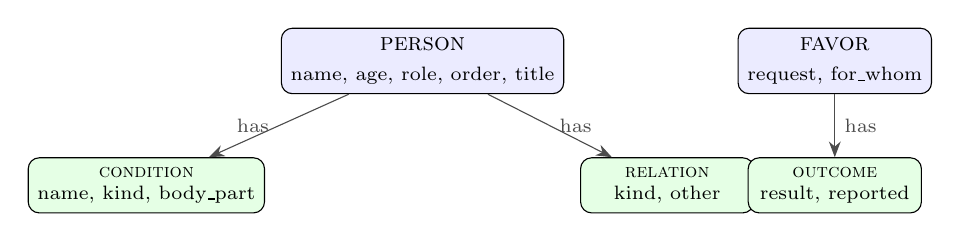
\begin{tikzpicture}[
   node distance=4mm and 10mm,
   t/.style={draw, rounded corners, fill=blue!8, align=center, font=\small,
             minimum width=24mm, minimum height=8mm},
   leaf/.style={draw, rounded corners, fill=green!10, align=center, font=\scriptsize,
                minimum width=22mm, minimum height=7mm},
   arr/.style={-{Stealth[length=2mm]}, gray!60!black}]

  \node[t] (person) {\type{person}\\\scriptsize name, age, role, order, title};
  \node[leaf, below left=8mm and 2mm of person] (cond)
       {\type{condition}\\name, kind, body\_part};
  \node[leaf, below right=8mm and 2mm of person] (rel)
       {\type{relation}\\kind, other};

  \node[t, right=22mm of person] (favor) {\type{favor}\\\scriptsize request, for\_whom};
  \node[leaf, below=8mm of favor] (out) {\type{outcome}\\result, reported};

  \draw[arr] (person) -- (cond) node[midway, left, font=\scriptsize] {has};
  \draw[arr] (person) -- (rel)  node[midway, right, font=\scriptsize] {has};
  \draw[arr] (favor)  -- (out)  node[midway, right, font=\scriptsize] {has};
\end{tikzpicture}
\caption{The schema is \emph{nested}: a \type{condition} and a \type{relation} can
hang off the \type{person} they belong to, and a \type{favor} carries its
\type{outcome} inline --- because in this corpus those facts arrive bundled. After
extraction, \code{\_flatten\_extraction()} also lifts each nested fact into its own
searchable mention, linked back with an \code{of\_person} / \code{for\_favor}
attribute.}
\end{figure}

\FloatBarrier

\subsection{GLiNER vs.\ the LLM: a two-tier extractor}

RESEARCH\_PLAN Part~B's ideal is two tiers: a \textbf{fine-tuned GLiNER} doing
fast, cheap, \emph{local} bulk NER over all $\sim$9k chunks, escalating only the
hard / low-confidence pages to Gemini. This stage implements the \textbf{LLM tier}
(the escalation target) end-to-end; GLiNER is the documented cheaper bulk path to
add later (custom types, nested spans, proven on historical documents).

\begin{center}
\small
\begin{tabular}{lll}
\toprule
 & GLiNER (bulk, future) & Gemini structured output (this stage) \\
\midrule
cost            & local, $\approx\$0$        & paid/token (batch $-50\%$, cache prefix) \\
shines on       & high-volume clean spans    & nested facts, world knowledge, messy prose \\
output guarantee& span offsets               & constrained-decoded valid JSON \\
role            & first pass on everything   & escalation for hard / low-conf pages \\
\bottomrule
\end{tabular}
\end{center}

\subsection{Coreference $\to$ relation $\to$ event: the KG trinity}

The frontier (LINK-KG, Extract-Define-Canonicalize, Relik) chains three steps:
resolve \textbf{coreference} (mentions $\to$ entities, within and across documents),
extract \textbf{relations} (\textsc{wrote\_to}, \textsc{enrolled\_for},
\textsc{located\_at}), then assemble \textbf{events} (an enrollment event, an
outcome event) with time + provenance. This stage \emph{seeds} all three: the
nested schema already captures relations and favour$\to$outcome event pairs
\emph{within} a passage; the resolver (next section) does the cross-document
coreference; full cross-passage relation/event extraction is the Part-C follow-up.

\subsection{Cost discipline (nothing bills by accident)}

\begin{cautionbox}[Paid work is deferred behind one switch]
By default the stage runs Pass~A for the whole corpus, \emph{previews} Pass~B
(builds the real prompt + schema, projects the cost), and logs a \$0 projection row
so even a dry run leaves a trace in \file{costs/usage.csv}. Only \code{execute=True}
(\code{-{}-execute}) spends a cent.
\end{cautionbox}

Two levers cut the real bill, both straight from RESEARCH\_PLAN Part~E:
\begin{itemize}[leftmargin=*]
  \item \textbf{Batch API} ($-50\%$, asynchronous, fine for an offline build).
        \code{write\_batch\_requests()} emits exactly the request file; submission
        is the deferred paid step.
  \item \textbf{Prompt caching} on the \emph{constant} \code{SYSTEM\_INSTRUCTION} +
        \code{response\_schema} prefix --- cached reads bill at $\approx 10\%$ of
        input price. See \code{build\_cache\_note()}.
\end{itemize}
Live runs are \textbf{idempotent and resumable}: \code{\_done\_unit\_ids()} skips any
unit already extracted, so a crash at unit 4{,}000 of 9{,}000 never re-pays. Every
real call routes through \code{lib.costlog.log(\dots)}.

% =============================================================================
\section{Entity resolution: the ``grouping,'' step by step}
% =============================================================================

\[
\text{normalize} \;\to\; \text{block} \;\to\; \text{match} \;\to\;
\text{cluster} \;\to\; \text{canonicalize} \;\to\; (\text{authority reconcile})
\]

The running example: the same human appears as \texttt{"Grace."},
\texttt{"Grace Panyard"}, \texttt{"Mrs.\ Grace Panyard"}; OCR turns
\texttt{O'Donnell} into \texttt{ODonnell}/\texttt{O Donnell}; a place is
\texttt{Detroit} here and \texttt{Detroit, Mich.}\ there. Resolution decides which
of those surface \emph{mentions} point at the same \emph{entity}.

\subsection{Step 1 --- Normalize: messy surface $\to$ stable keys}

We never \emph{fix} the text (the original surface is preserved); we only derive
\emph{stable comparison keys}. \code{normalize\_tokens()} folds accents,
lower-cases, splits punctuation (so \texttt{O'Donnell}, \texttt{O`Donnell},
\texttt{ODonnell}, \texttt{O Donnell} all become the tokens \texttt{[o, donnell]}),
strips honorifics (\texttt{mrs}, \texttt{fr}), and expands abbreviations
(\texttt{st}$\to$\texttt{saint}, \texttt{mich}$\to$\texttt{michigan}). Then
\textbf{Double Metaphone} encodes each token by how it \emph{sounds}, so spellings
that differ only in silent letters or OCR slips collide (\texttt{Panyard} and
\texttt{Panyord} share a code).

\begin{primerbox}[Why phonetics, and why \emph{two} keys]
A phonetic code maps a word to how it sounds. \code{phonetic\_key} encodes the
tokens \emph{one at a time}; \code{phonetic\_key\_joined} encodes the tokens
\emph{concatenated} (``odonnell'') as one word. We need both because a name one
scribe wrote as a single token and another split into two would get different
\emph{per-token} keys --- but identical \emph{joined} keys --- so the joined key is
the bridge that keeps those genuinely-equal surfaces in the same bucket. The module
\textbf{vendors} a compact, dependency-free Double Metaphone so the stage runs with
zero installs; \code{\_phonetic()} automatically prefers the \code{metaphone} /
\code{jellyfish} package if present.
\end{primerbox}

\subsection{Step 2 --- Block: cheap candidate generation (avoid \texorpdfstring{$O(n^2)$}{O(n2)})}

\begin{figure}[h]
\centering
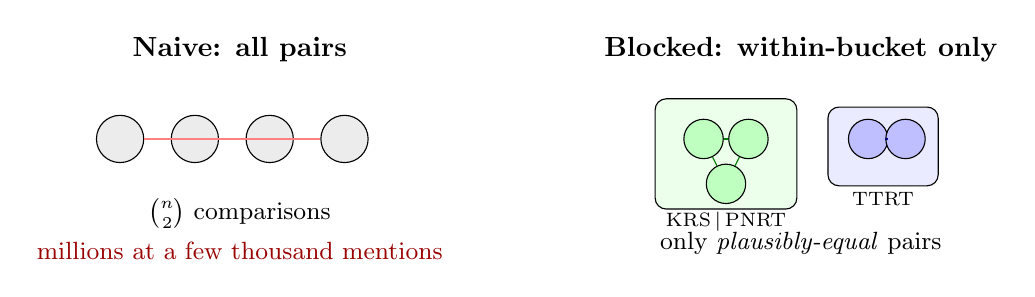
\begin{tikzpicture}[scale=0.95, every node/.style={font=\small}]
  % left: all-pairs
  \node[font=\bfseries] at (1.6,2.6) {Naive: all pairs};
  \foreach \i in {0,1,2,3} {
    \node[circle, draw, fill=gray!15, minimum size=6mm] (L\i) at (\i,1.4) {};
  }
  \foreach \i in {0,1,2,3} \foreach \j in {0,1,2,3} {
    \ifnum\i<\j \draw[red!50] (L\i) -- (L\j); \fi
  }
  \node at (1.6,0.4) {$\binom{n}{2}$ comparisons};
  \node[font=\small, red!60!black] at (1.6,-0.1) {millions at a few thousand mentions};

  % right: blocked
  \begin{scope}[xshift=7.5cm]
    \node[font=\bfseries] at (1.6,2.6) {Blocked: within-bucket only};
    % bucket 1 (Grace)
    \node[draw, rounded corners, fill=green!8, minimum width=18mm, minimum height=14mm]
         (b1) at (0.6,1.2) {};
    \node[circle, draw, fill=green!25, minimum size=5mm] (g0) at (0.3,1.4) {};
    \node[circle, draw, fill=green!25, minimum size=5mm] (g1) at (0.9,1.4) {};
    \node[circle, draw, fill=green!25, minimum size=5mm] (g2) at (0.6,0.8) {};
    \draw[green!50!black] (g0)--(g1); \draw[green!50!black] (g1)--(g2); \draw[green!50!black] (g0)--(g2);
    \node[font=\scriptsize] at (0.6,0.3) {KRS\,$\vert$\,PNRT};
    % bucket 2 (Detroit)
    \node[draw, rounded corners, fill=blue!8, minimum width=14mm, minimum height=10mm]
         (b2) at (2.7,1.3) {};
    \node[circle, draw, fill=blue!25, minimum size=5mm] (d0) at (2.5,1.4) {};
    \node[circle, draw, fill=blue!25, minimum size=5mm] (d1) at (3.0,1.4) {};
    \draw[blue!50!black] (d0)--(d1);
    \node[font=\scriptsize] at (2.7,0.6) {TTRT};
    \node at (1.6,0.0) {only \emph{plausibly-equal} pairs};
  \end{scope}
\end{tikzpicture}
\caption{Blocking is why resolution is fast. Bucket mentions by a cheap key
(\code{type:phonetic[:location][:year]}) and compare only \emph{within} a bucket.
``Grace'' never gets compared against ``Detroit.'' Each mention emits several keys
(multi-pass / canopy blocking) and we union the candidates, so a real match
survives even if one record lacks a city.}
\end{figure}

\FloatBarrier

A subtle key (\code{phj=}) encodes the \emph{joined} tokens, so a name split
differently by two scribes still meets in a shared bucket --- without it, blocking
would propose the pair but the matcher would never see it.

\subsection{Step 3 --- Match: an ensemble of \emph{interpretable} signals}

Within a block, \code{pair\_score()} scores each pair on cheap, interpretable
features --- interpretable beats a black box here, because David must be able to
read the audit log and agree or disagree with each merge.

\begin{center}
\small
\begin{tabular}{lcl}
\toprule
signal & weight & catches \\
\midrule
phonetic equality      & 0.35 & same-sounding OCR / spelling variants \\
Levenshtein ratio      & 0.30 & single-character slips (\texttt{panyard} vs \texttt{panyord}) \\
token Jaccard          & 0.20 & reordering / extra tokens \\
attribute agreement    & 0.15 & same city / role / order where both supply it \\
embedding cosine       & \emph{bonus} & \emph{semantic} nearness (gated; blended, not replacing) \\
\bottomrule
\end{tabular}
\end{center}

\[
\text{score} \;=\; 0.35\,\mathrm{ph} \;+\; 0.30\,\mathrm{lev} \;+\;
0.20\,\mathrm{jac} \;+\; 0.15\,\mathrm{agree},
\]
clamped to $[0,1]$. When the gated embedding signal is present it blends in as
$0.85\cdot\text{score} + 0.15\cdot\cos$, so the decision stays \emph{mostly}
interpretable. Levenshtein is computed on the \emph{spaceless} normalized forms so
a stray OCR space doesn't penalize an otherwise-identical name; attribute agreement
is a neutral $0.5$ when neither record supplies the attribute.

\subsection{Step 4 --- Cluster: agreeing pairs $\to$ entities}

Pairwise matches form a graph --- mentions are nodes, an edge joins a pair scoring
above \code{MATCH\_TAU}. An \textbf{entity} is a \emph{connected component}: if
$A\!\sim\!B$ and $B\!\sim\!C$, then $A,B,C$ are one entity (transitive closure). A
tiny union-find (\code{\_UnionFind}, path compression + union by rank) computes this
in near-linear time, no graph library.

\begin{center}
\small
\begin{tabular}{ll}
\toprule
threshold & meaning \\
\midrule
\code{MATCH\_TAU = 0.62} & $\ge$: confident same-entity edge (merge) \\
\code{AMBIG\_TAU = 0.50} & $[\,0.50, 0.62)$: grey zone $\to$ flag for review / LLM \\
\bottomrule
\end{tabular}
\end{center}

Any component touched by a grey edge is flagged \emph{ambiguous} and, if enabled,
sent to LLM adjudication; otherwise it goes straight to David's review queue. The
thresholds deliberately favour \textbf{precision} (see Caveats).

\subsection{Step 5 --- Canonicalize: one authority record per entity}

\code{canonicalize()} turns each component into one record: pick the fullest,
best-attested surface as \code{canonical\_name} (``Grace Panyard'' beats ``Grace.''
--- more tokens, tie-broken by frequency), collect every distinct surface as
\code{variants[]}, majority-vote the attributes, gather every mention's provenance,
and compute a \code{confidence} that blends internal name agreement with the OCR
\code{min\_conf} of the source regions. \code{needs\_review} marks the grey clusters.

\begin{lstlisting}[language=,caption={A canonical record (data/entities.json).}]
{
  "id": "person:grace_panyard:0007",
  "type": "PERSON",
  "canonical_name": "Grace Panyard",
  "variants": ["Grace.", "Grace Panyard", "Mrs. Grace Panyard"],
  "attrs": {"city": "Detroit"},
  "mentions": [
    {"mention_id": "...", "surface": "Grace.",
     "provenance": {"doc_id": "...", "rid": "...", "page": 3,
                    "vertices": [[x,y],[x,y],[x,y],[x,y]], "min_conf": 0.948}}
  ],
  "confidence": 0.91,
  "needs_review": false,
  "authority": {"wikidata": null, "viaf": null, "geonames": null, "getty_tgn": null}
}
\end{lstlisting}

% =============================================================================
\section{The three gated power-ups}
% =============================================================================

Each is a real function with a \code{gated=True} guard, a clear TODO, and
cost-logging --- wired and documented, but \textbf{never run by default}.

\begin{enumerate}[leftmargin=*]
  \item \textbf{Embedding similarity} (\code{embedding\_signal}). Cosine over mention
        embeddings, computed \emph{only} for the pairs blocking already proposed
        (never full $n^2$). Phonetics are blind to \emph{meaning}: ``the Capuchin
        friary at Harlem'' and ``St.\ Bonaventure Monastery'' share no characters
        but embed near each other. Routes through \code{lib.providers.embed}; the
        \emph{free local} path (\code{bge-small}, \$0) is the default, paid spaces
        are key-gated.
  \item \textbf{LLM adjudication} (\code{llm\_adjudicate}). Only on clusters flagged
        ambiguous, the model returns a \emph{structured} keep/split verdict
        (auditable, not prose). This is the 2025-SOTA tiebreaker (in-context
        clustering / LLM-as-judge, $\sim$94\% on name variants). A \code{split}
        verdict is \emph{recorded in the audit, not auto-applied} --- David reviews
        before any re-partition.
  \item \textbf{Authority reconciliation} (\code{reconcile\_person},
        \code{reconcile\_place}). Link persons $\to$ \textbf{Wikidata/VIAF}, places
        $\to$ \textbf{GeoNames/Getty TGN}, for global IDs, disambiguation,
        enrichment, and Linked-Data export. These public APIs don't bill, but every
        call is still cost-logged at \$0 so the ledger is complete.
\end{enumerate}

% =============================================================================
\section{Scale-up path: Splink}
% =============================================================================

For a \emph{much} larger corpus, \code{splink\_plan()} documents the drop-in swap to
\textbf{Splink} (probabilistic record linkage; Fellegi--Sunter with EM-learned match
weights; DuckDB/Spark; millions of records on a laptop). Our pieces map almost
one-to-one, so this is a scale path, not a rewrite:

\begin{center}
\small
\begin{tabular}{ll}
\toprule
this module & Splink \\
\midrule
\code{blocking\_keys()}     & \code{blocking\_rules\_to\_generate\_predictions} \\
\code{pair\_score()} signals & \code{comparisons} / \code{ComparisonLevel}s (jaro\_winkler, exact, custom-sql) \\
\code{cluster\_mentions()}  & \code{cluster\_pairwise\_predictions\_at\_threshold} \\
\bottomrule
\end{tabular}
\end{center}

Precompute the \code{phonetic\_key} / \code{norm\_name} columns with this module's
functions and feed them to Splink, so blocking and comparisons reuse exactly the
same normalization.

% =============================================================================
\section{How to run}
% =============================================================================

\begin{lstlisting}[language=bash]
# from step_7/ with the venv active

# NER -- free Pass A + a no-spend preview of Pass B
python stages/extract_entities.py --limit 25
python stages/extract_entities.py --batch     # emit Gemini Batch file (no spend)
python stages/extract_entities.py --execute   # PAID live LLM pass (authorize first)

# Resolution -- offline rule-based core ($0)
python stages/resolve_entities.py
python stages/resolve_entities.py --use-embeddings   # free local bge by default
python stages/resolve_entities.py --use-llm          # GATED; bills tokens
python stages/resolve_entities.py --reconcile        # Wikidata/VIAF/GeoNames/Getty ($0)
\end{lstlisting}

\noindent\textbf{Artifacts} (all new files --- non-destructive):
\file{data/entities\_raw.jsonl} (mentions), \file{data/entities.json} (canonical
records + \code{\_meta}), \file{data/entities\_merge\_audit.jsonl} (one row per merge
decision), \file{data/entities\_batch\_requests.jsonl} (optional batch file).

% =============================================================================
\section{Caveats}
% =============================================================================

\begin{cautionbox}[Read before trusting a run at scale]
\begin{itemize}[leftmargin=*]
  \item \textbf{A wrong merge is worse than a wrong split.} Merging two real people
        pollutes every query about either; a split merely scatters one person across
        two records. Thresholds therefore favour precision, and the grey zone routes
        to review. Tune \code{MATCH\_TAU} / \code{AMBIG\_TAU} on David's gold first.
  \item \textbf{Mention-schema seam between the two stages.}
        \code{extract\_entities.py} currently emits mentions keyed \code{text} /
        \code{unit\_id} / \code{pass}, while \code{resolve\_entities.py} reads
        \code{surface} / \code{mention\_id} (its SCHEMA block documents the expected
        contract). Until a tiny adapter bridges them, the resolver runs on its
        \emph{demo fallback} (recipient names from the letters' structured fields),
        clearly labelled in the output \code{\_meta.source}. A known, small
        follow-up --- flagged so the next run isn't surprised.
  \item \textbf{Pass~B is deferred.} No live extraction has run; Pass-B figures are
        projections. Schema, prompt, batch file, and resume logic are real and
        dry-run tested.
  \item \textbf{The vendored Double Metaphone is a pragmatic subset} (high-value
        rules, not Philips' full $\sim$250-line algorithm) --- good enough for
        blocking; install \code{metaphone}/\code{jellyfish} for the full version.
  \item \textbf{The LLM \code{split} verdict isn't auto-applied} yet; it is recorded
        for review. Authority lookups are best-effort and never crash a run.
  \item \textbf{Prices are placeholders.} Confirm provider pricing before any billed
        run; nothing bills until a stage is explicitly executed.
\end{itemize}
\end{cautionbox}

% =============================================================================
\section{Sources}
% =============================================================================

\begin{itemize}[leftmargin=*]
  \item \textbf{GLiNER} (custom + nested NER): \url{https://github.com/urchade/GLiNER};
        fine-tuning generalist NER:
        \url{https://labelstud.io/blog/fine-tuning-generalist-models-for-named-entity-recognition/};
        historical NER (Zibaldone): \url{https://arxiv.org/pdf/2505.20113}.
  \item \textbf{Structured / constrained output}: Outlines on AWS
        \url{https://aws.amazon.com/blogs/machine-learning/generate-structured-output-from-llms-with-dottxt-outlines-in-aws/};
        JSONSchemaBench \url{https://arxiv.org/pdf/2501.10868}.
  \item \textbf{Coref $\to$ relation $\to$ event $\to$ KG}: LINK-KG
        \url{https://arxiv.org/html/2510.26486}; Extract-Define-Canonicalize
        \url{https://arxiv.org/pdf/2404.03868}; Relik
        \url{https://neo4j.com/blog/developer/entity-linking-relationship-extraction-relik-llamaindex/}.
  \item \textbf{Entity resolution}: Splink
        \url{https://github.com/moj-analytical-services/splink}; ER intro
        \url{https://medium.com/@adev94/entity-resolution-an-introduction-fb2394d9a04e};
        LLM in-context clustering ER \url{https://arxiv.org/abs/2506.02509}.
  \item \textbf{Authority control}: Wikidata, VIAF, GeoNames, Getty TGN public
        reconciliation endpoints.
  \item \textbf{Cost}: prompt caching 2026
        \url{https://www.digitalapplied.com/blog/prompt-caching-2026-cut-llm-costs-engineering-guide};
        Gemini pricing \url{https://costbench.com/software/llm-api-providers/google-gemini-api/}.
\end{itemize}

\end{document}
</content>
